\section{The potential}
\label{sec-potential}

You can specify a potential in rectangular, polar, or complex
coordinates. Here are some examples.

\begin{figure}[h!]
 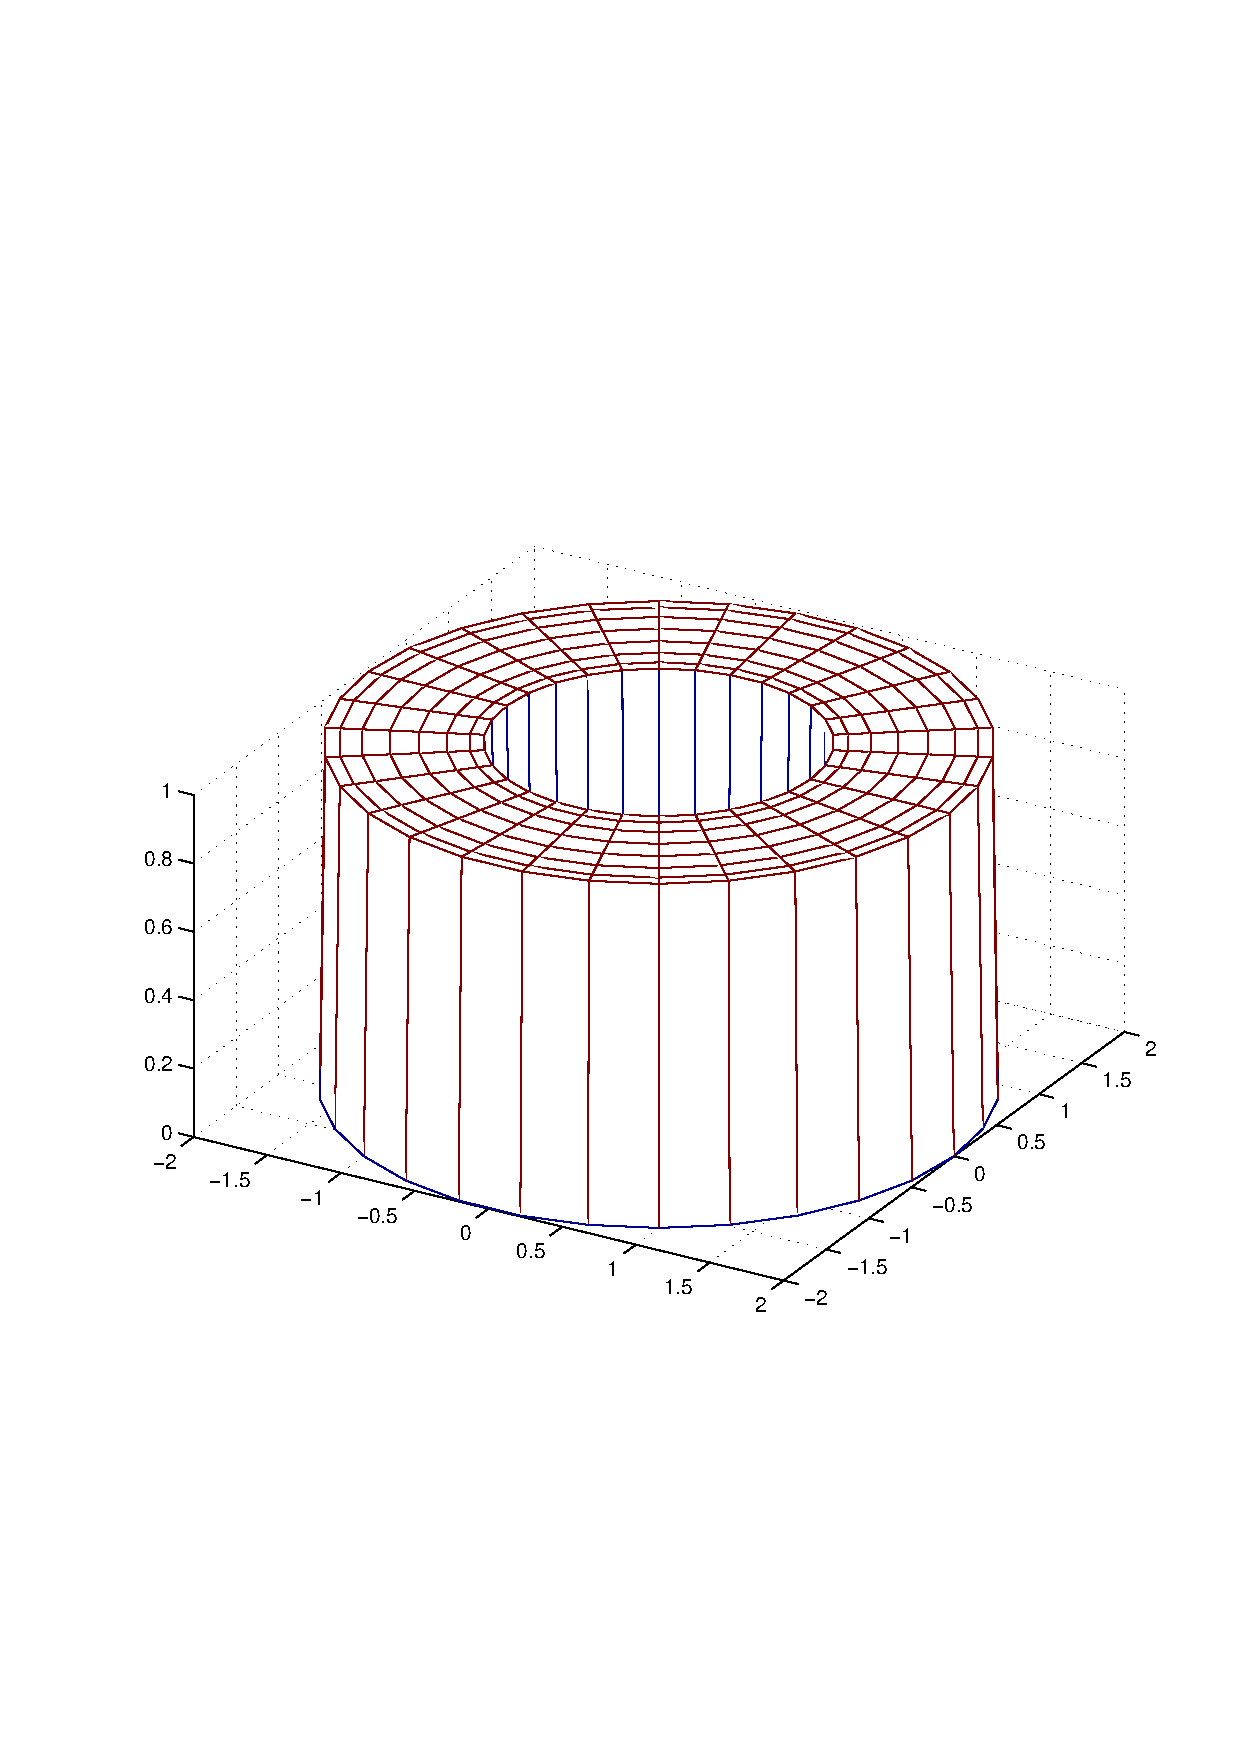
\includegraphics[width=0.55\linewidth]{figures/ringpotential.pdf}
 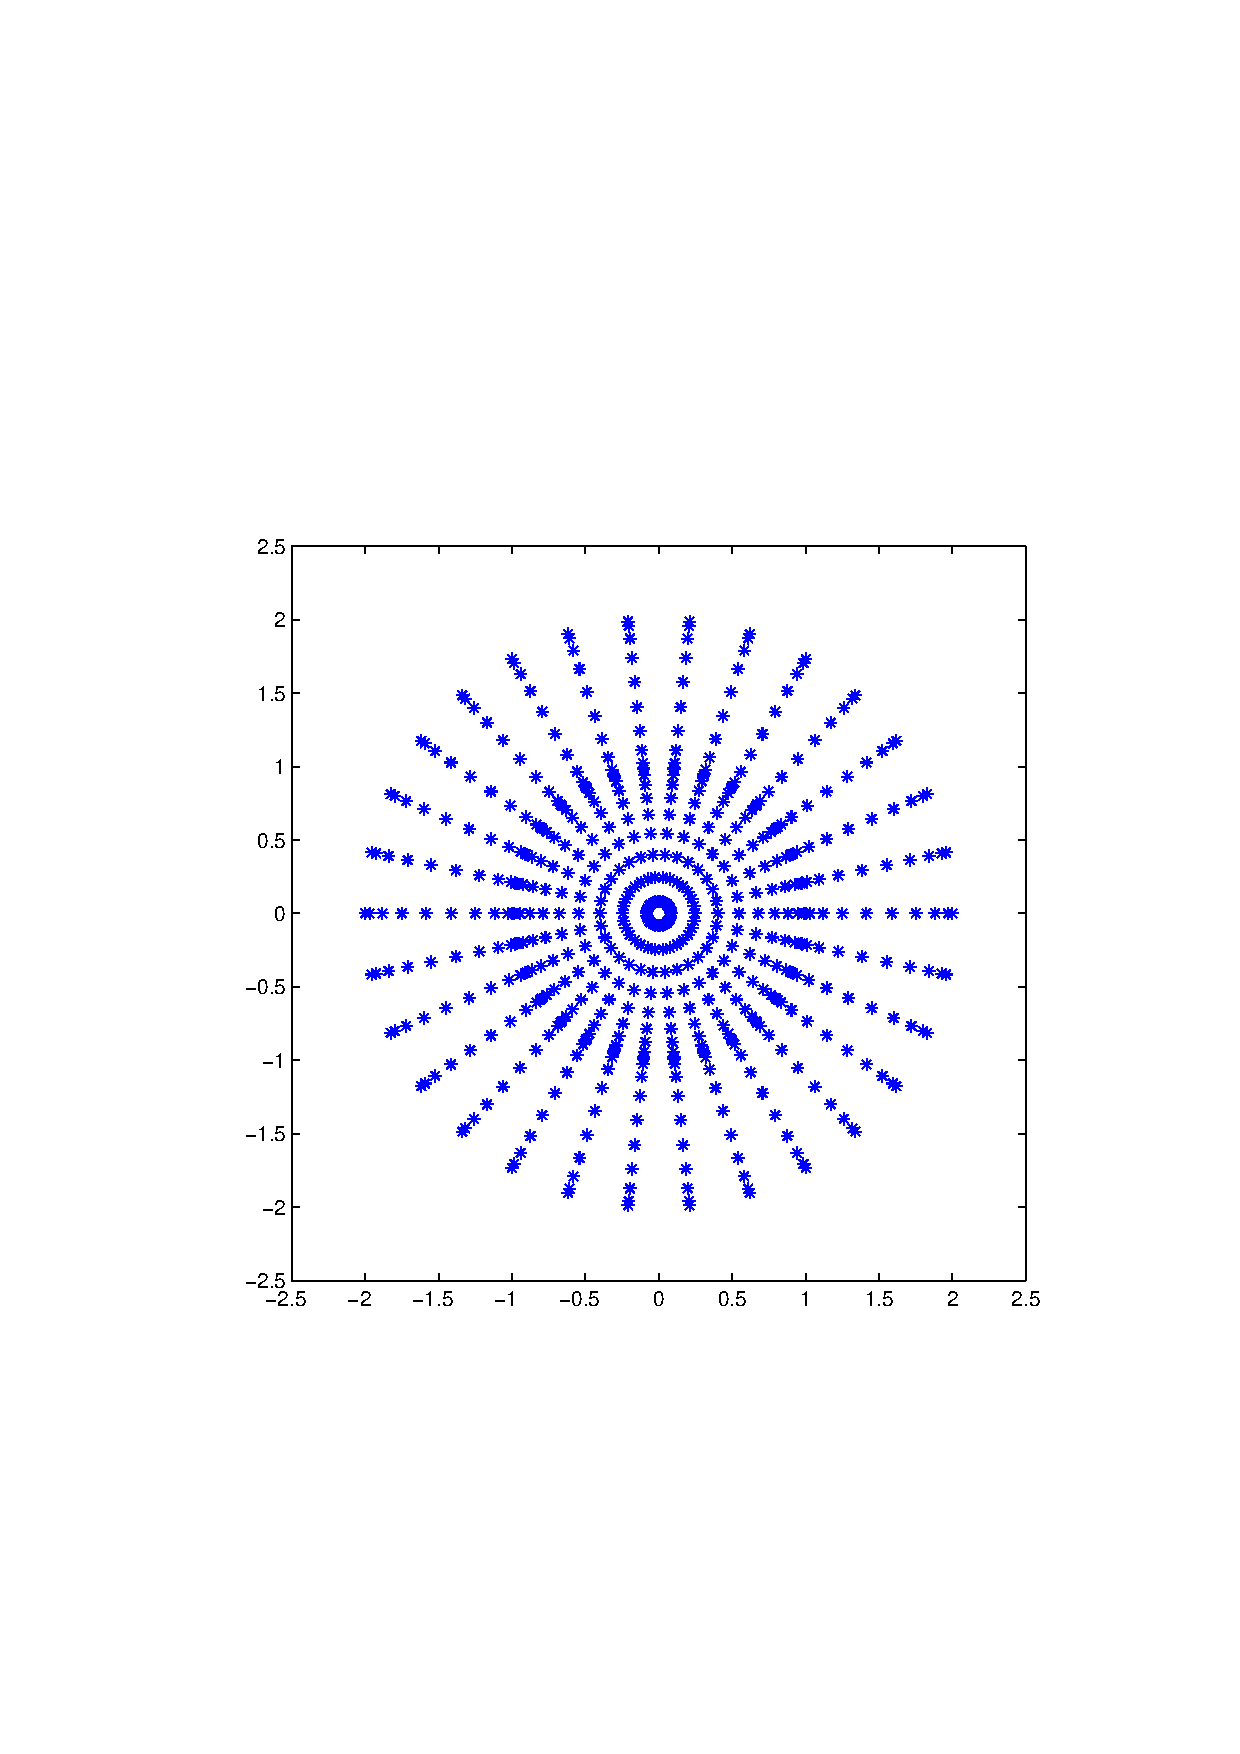
\includegraphics[width=0.45\linewidth]{figures/ringpotentialmesh.pdf} \\ 
 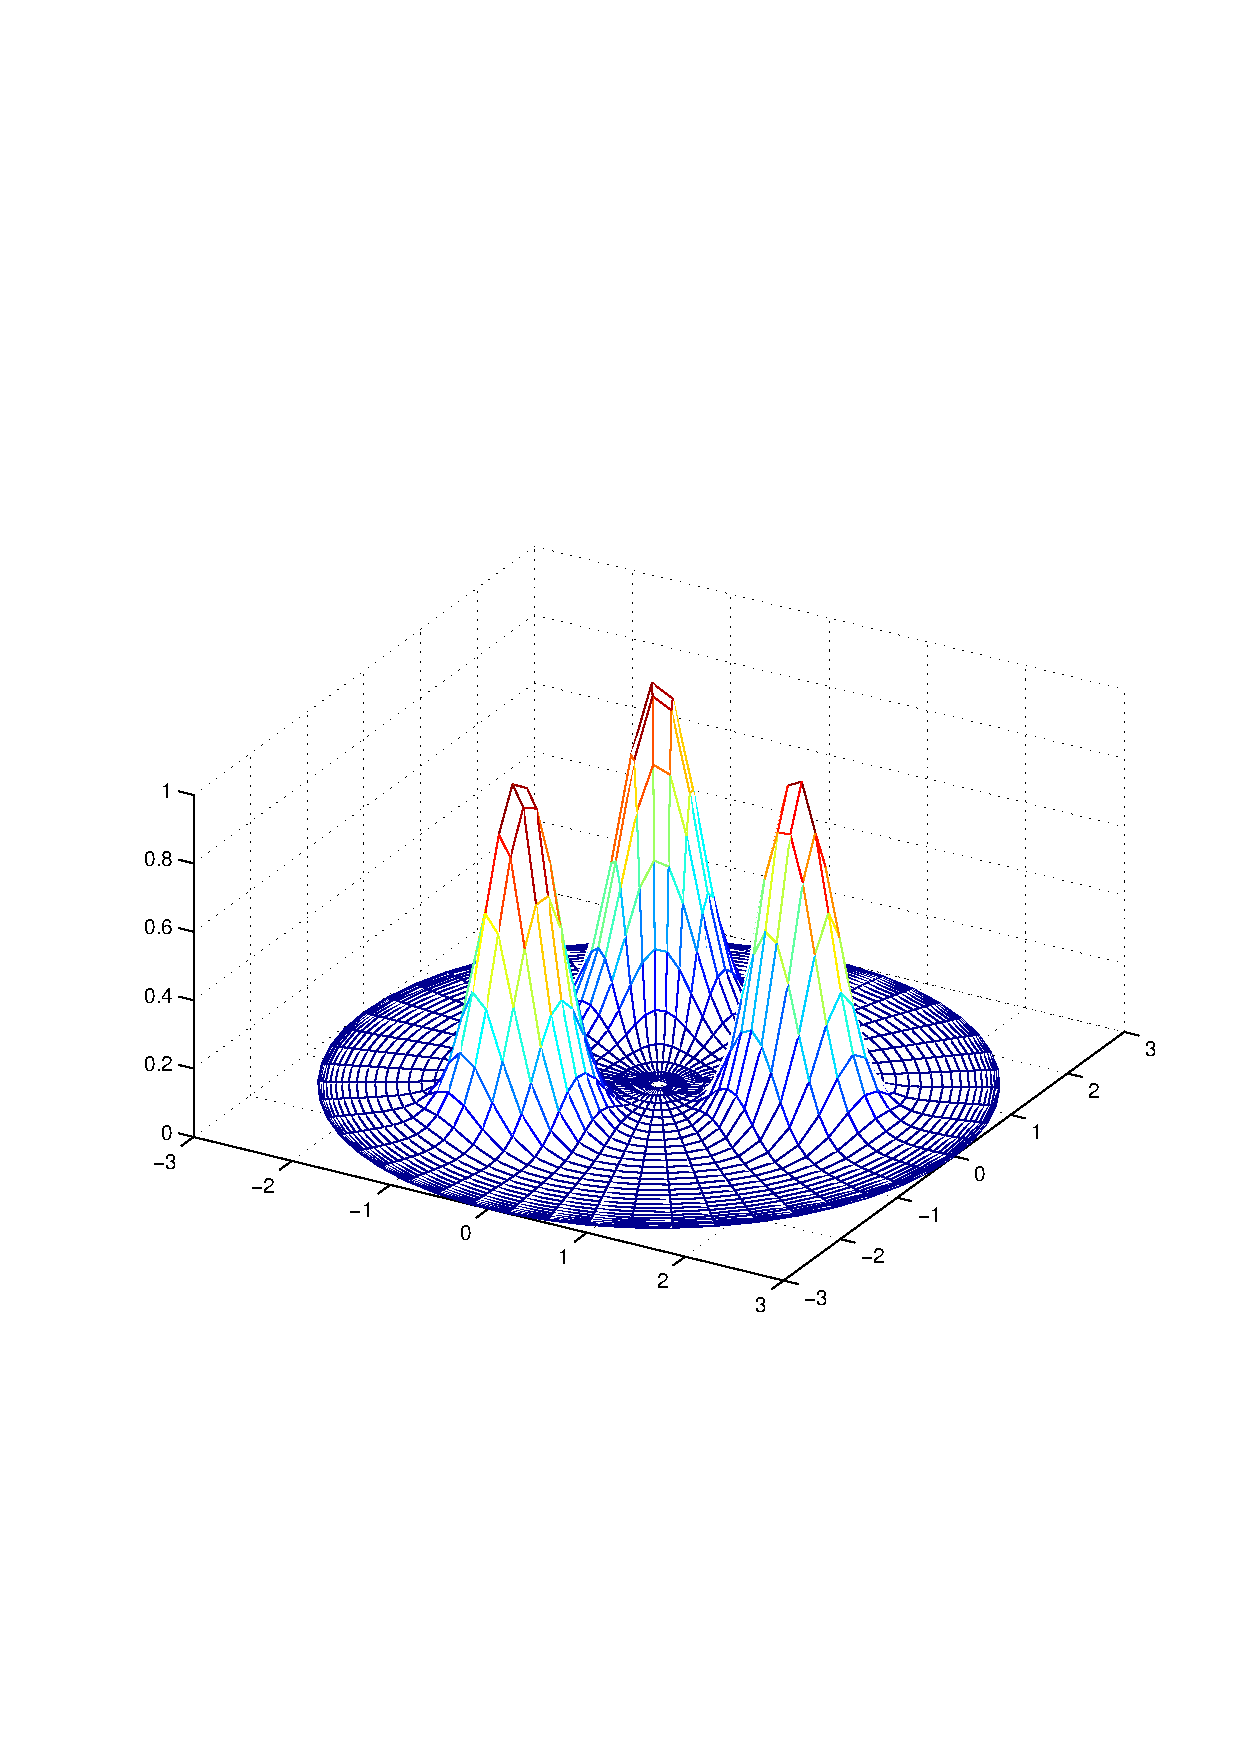
\includegraphics[width=0.55\linewidth]{figures/threebumppotential.pdf}
 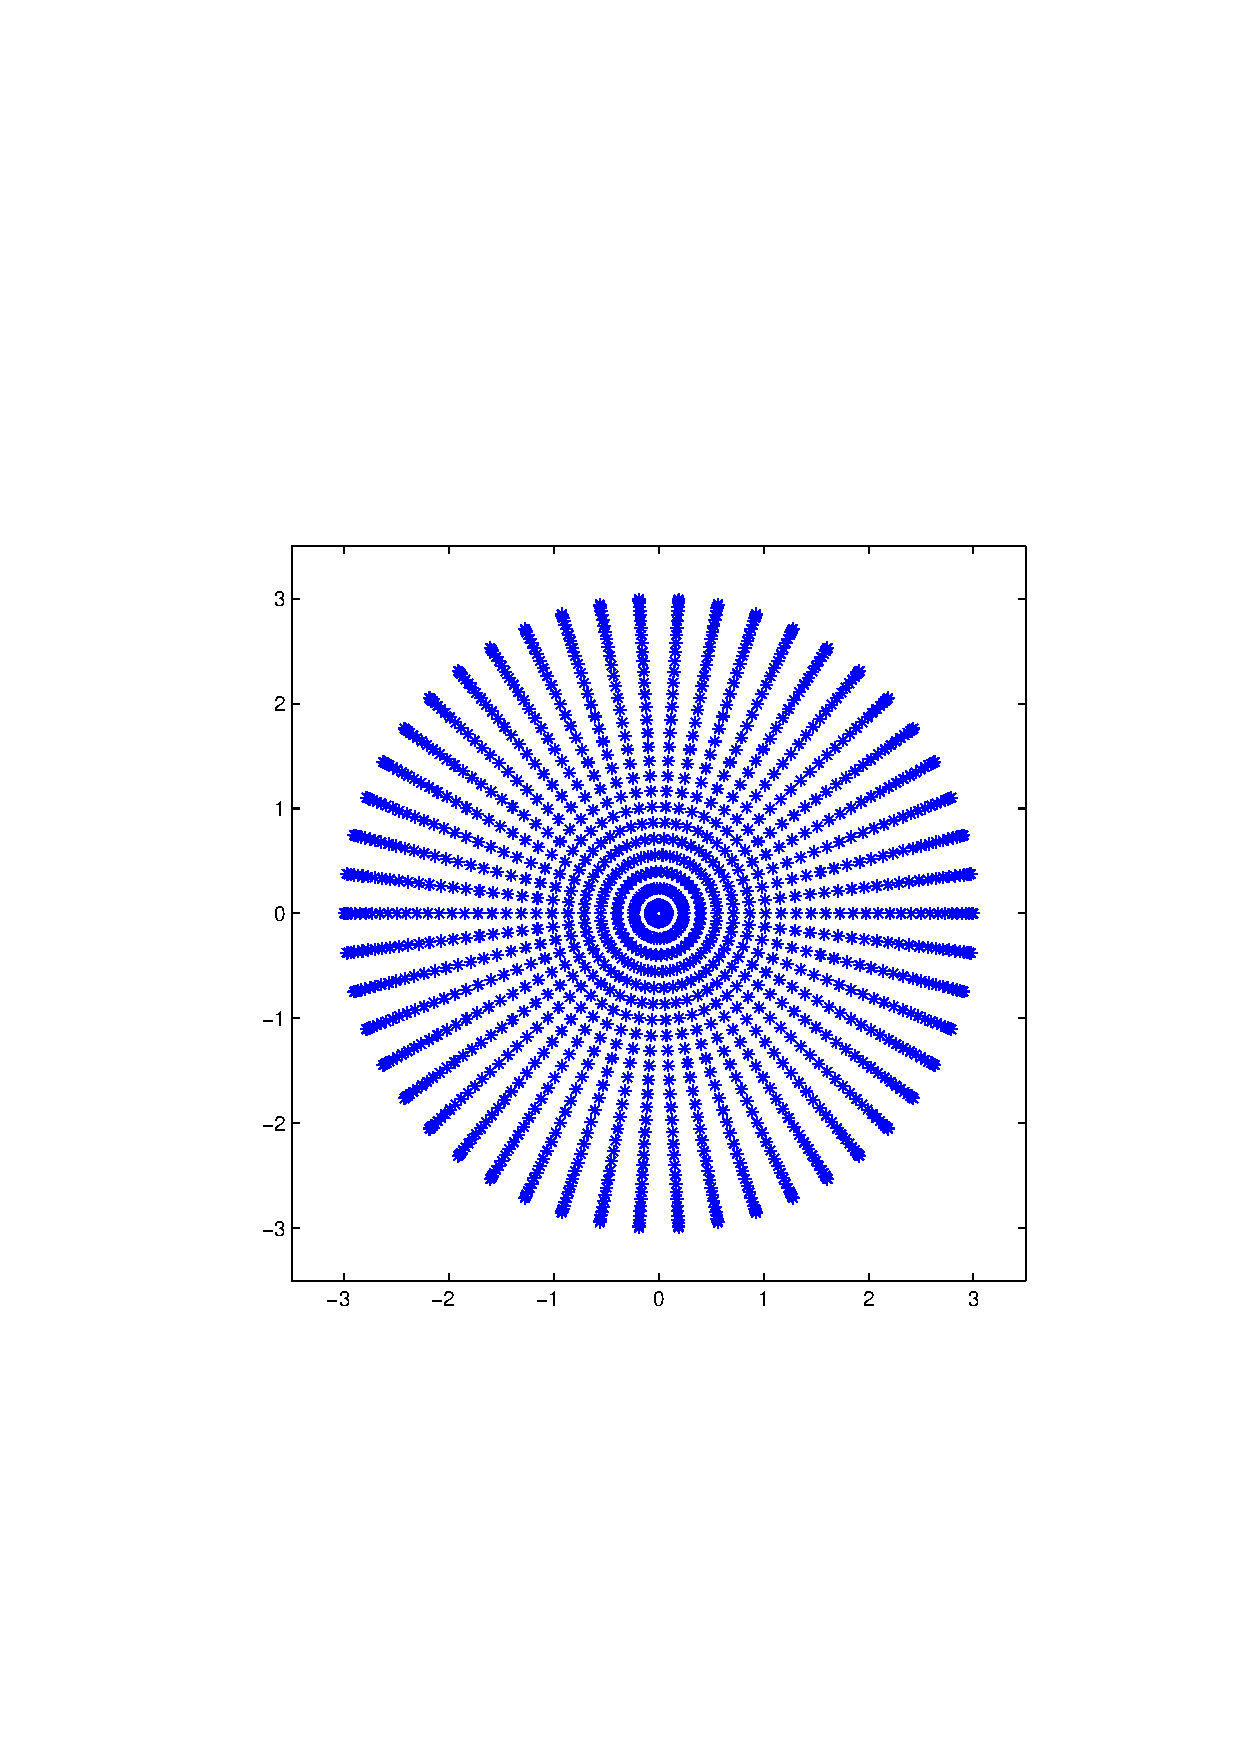
\includegraphics[width=0.45\linewidth]{figures/threebumppotentialmesh.pdf}
 \caption{Top Left: An axisymmetric, piecewise constant potential
                equal to 1 on $1 < r < 2$ and zero elsewhere.
          Top Right: The regions where the potential is constant
                 must be meshed separately.
          Bottom Left: A potential consisting of three bumps. Most
                 of the volume of the potential is contained in
                 $B(0,3)$.
          Bottom Right: Since the potential function is continuous
                 everywhere, the disc $B(0,3)$ can be meshed without
                 splitting it into a central disk and annular regions.}
\end{figure}
